% =============================================================================================
\chapter{Résultats}\label{chap:resultats}

% ---------------------------------------------------------------------------------------------
\section{Modèle de risque}

\subsection{Comparaison des trois modèles}

Le tableau~\ref{tab:modeles} donne les performances des versions calibrées. Sur le test, lu une seule fois, LightGBM
obtient la meilleure AUROC (0,800), devant l'EBM (0,778) et la régression logistique (0,726). Le même ordre se retrouve
en AUPRC (0,200, 0,170 et 0,159, pour un taux de défaut de 4,25\,\%, donc environ quatre à cinq fois mieux que le
hasard) et en F1.

\begin{table}[htbp]
\centering
\footnotesize\setlength{\tabcolsep}{4pt}
\caption{Performances des trois modèles (versions calibrées). Taux de défaut réel : 3,57\,\% en validation, 4,25\,\% en test}\label{tab:modeles}
\begin{tabular}{lccccccc}
\toprule
Modèle (calibré) & AUROC val. & Brier val. & AUROC test & AUPRC test & F1 test & Brier test & PD moy. test \\
\midrule
Régression logistique & 0,733 & 0,0325 & 0,726 & 0,159 & 0,239 & 0,0380 & 3,67\,\% \\
\textbf{EBM (retenu)} & 0,767 & 0,0325 & 0,778 & 0,170 & 0,247 & 0,0379 & 3,52\,\% \\
LightGBM (référence) & 0,793 & 0,0318 & 0,800 & 0,200 & 0,282 & 0,0370 & 3,59\,\% \\
\bottomrule
\end{tabular}
\end{table}


\begin{encadre}[Le prix de l'interprétabilité]
La règle de choix, fixée avant l'entraînement de LightGBM, retient l'\textbf{EBM}, meilleur modèle interprétable sur
la validation (Brier calibré de 0,03248 contre 0,03249 pour la logistique, et une AUROC nettement supérieure). L'écart
entre l'EBM et LightGBM sur le test est de 0,022 point d'AUROC et 0,030 point d'AUPRC, alors que l'EBM dépasse la
baseline de 0,052 point d'AUROC. Autrement dit, le modèle interprétable récupère environ 70\,\% du gain apporté par le
modèle opaque par rapport à la baseline. Pour une décision de crédit qui doit être justifiée, ce prix est faible.
\end{encadre}

\subsection{Calibration}

La figure~\ref{fig:calibration} compare les courbes de calibration. Sur la validation, les trois modèles calibrés
suivent la diagonale, ce qui est attendu puisque la calibration y est ajustée (de façon croisée pour la mesure). Sur
le test, les courbes restent proches de la diagonale pour les probabilités inférieures à 5\,\%, où se trouvent la
plupart des prêts, mais passent au-dessus pour les risques les plus élevés : les modèles sous-estiment le risque des
prêts les plus fragiles de 2015-2016. En moyenne, l'EBM prédit 3,52\,\% de défauts pour un taux réel de 4,25\,\%. Ce
léger décalage reflète la dérive entre périodes (le taux de défaut remonte de 3,6 à 4,3\,\% entre la validation et le
test) ; il conduit à une estimation un peu optimiste du risque, à garder à l'esprit dans l'interprétation.

\begin{figure}[htbp]
  \centering
  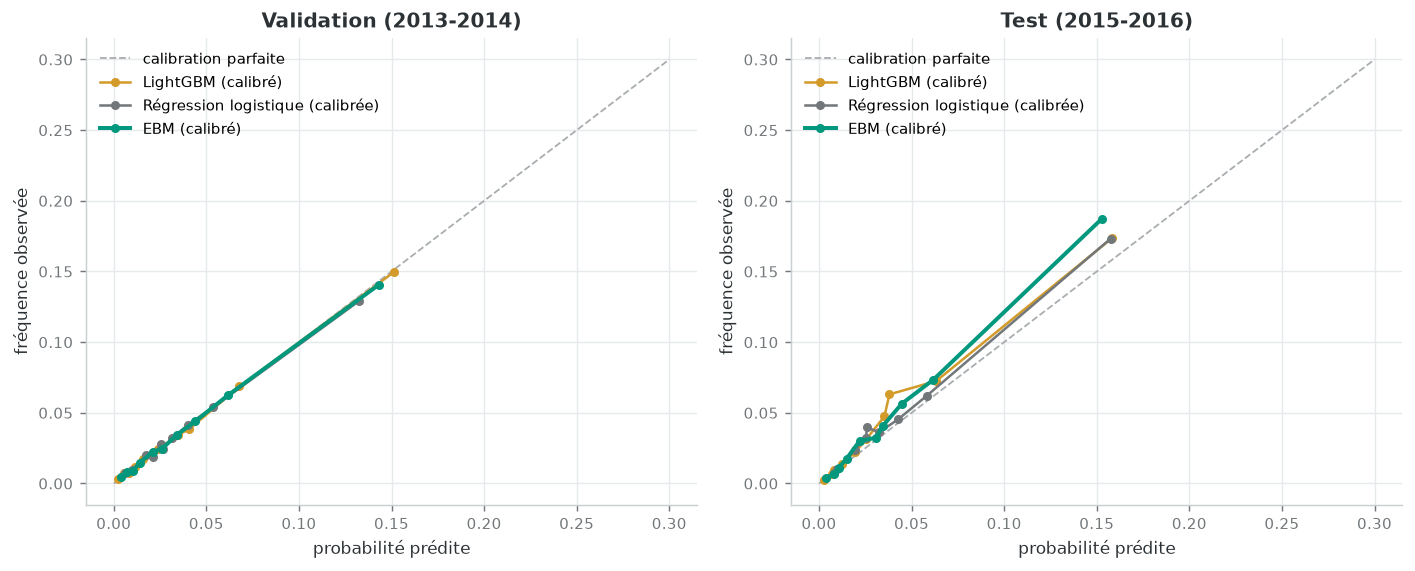
\includegraphics[width=\textwidth]{calibration.png}
  \caption{Courbes de calibration des trois modèles calibrés, sur la validation et sur le test (déciles de
  probabilité prédite).}
  \label{fig:calibration}
\end{figure}

\subsection{Interprétabilité}

\paragraph{Importance des variables.} L'importance par permutation de l'EBM et les valeurs SHAP de LightGBM
(tableau~\ref{tab:importance}, figures~\ref{fig:importance} et~\ref{fig:shap}) désignent les mêmes variables
principales : la tranche de durée et le taux d'intérêt initial, puis le montant, la procédure, l'État et la ligne
renouvelable. Mélanger la tranche de durée fait perdre 0,189 point d'AUROC à l'EBM, dix fois plus que toute autre
variable. Deux modèles de natures différentes s'accordant sur les facteurs de risque, ces résultats sont robustes.

\begin{table}[htbp]
\centering
\footnotesize\setlength{\tabcolsep}{4pt}
\caption{Importance des variables sur la validation : permutation pour l'EBM, valeurs SHAP pour LightGBM}\label{tab:importance}
\begin{tabular}{lccc}
\toprule
Variable & Baisse d'AUROC (EBM) & Écart-type & $|$SHAP$|$ moyen (LightGBM) \\
\midrule
tranche de durée & 0,1887 & 0,0080 & 0,723 \\
taux d'intérêt initial & 0,0295 & 0,0027 & 0,809 \\
montant (log) & 0,0270 & 0,0038 & 0,146 \\
ligne renouvelable & 0,0229 & 0,0017 & 0,069 \\
procédure SBA & 0,0170 & 0,0007 & 0,150 \\
État & 0,0116 & 0,0022 & 0,208 \\
taux fixe ou variable & 0,0088 & 0,0011 & 0,100 \\
secteur NAICS & 0,0084 & 0,0013 & 0,174 \\
part garantie SBA & 0,0028 & 0,0009 & 0,076 \\
type d'entreprise & 0,0005 & 0,0005 & 0,022 \\
franchise & 0,0001 & 0,0002 & 0,004 \\
taux non renseigné & 0,0000 & 0,0000 & 0,164 \\
âge de l'entreprise & -0,0002 & 0,0011 & 0,120 \\
\bottomrule
\end{tabular}
\end{table}


\begin{figure}[htbp]
  \centering
  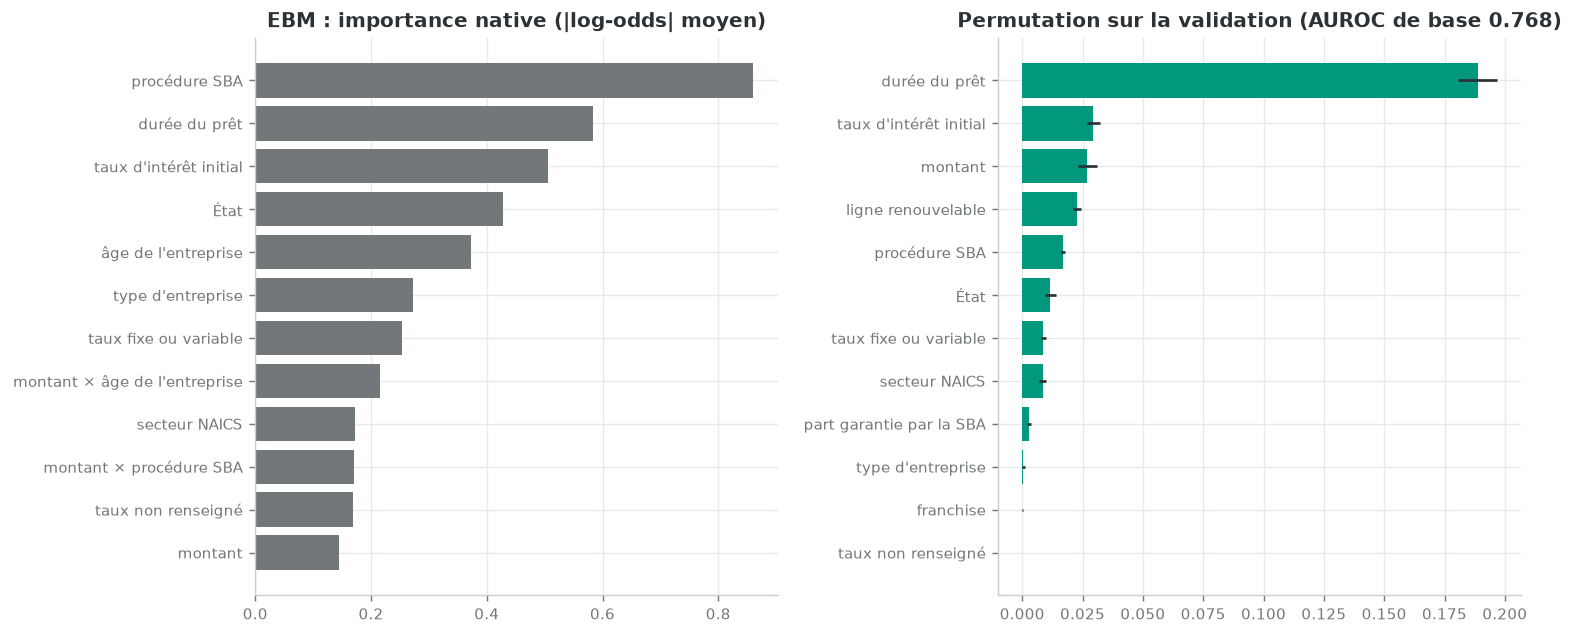
\includegraphics[width=\textwidth]{importance_variables.png}
  \caption{Importance native de l'EBM (contribution absolue moyenne, à gauche) et importance par permutation sur la
  validation (baisse d'AUROC, à droite).}
  \label{fig:importance}
\end{figure}

\begin{figure}[htbp]
  \centering
  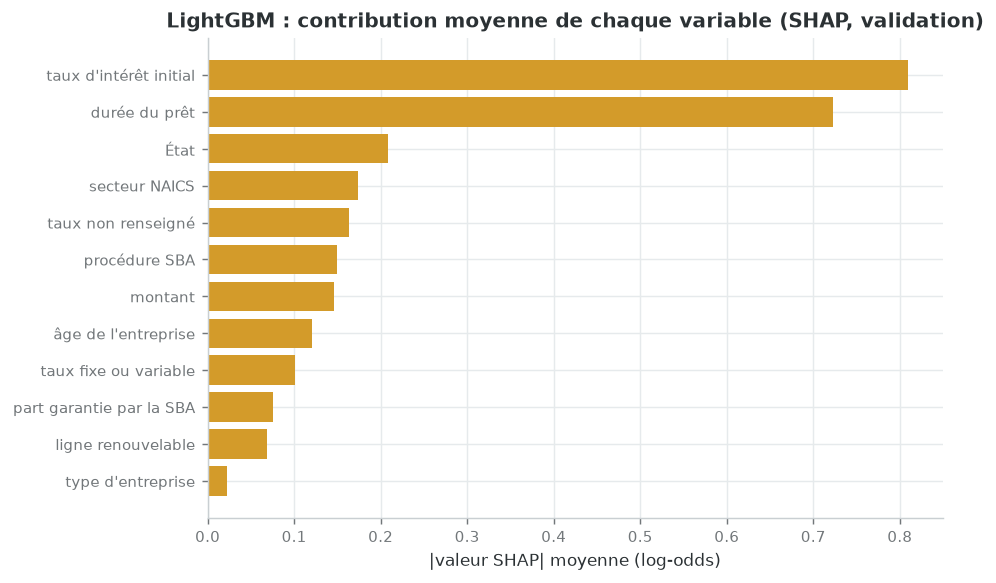
\includegraphics[width=0.75\textwidth]{shap_lightgbm.png}
  \caption{LightGBM : valeur SHAP absolue moyenne par variable (5\,000 prêts de validation).}
  \label{fig:shap}
\end{figure}

\paragraph{Effet des variables.} La figure~\ref{fig:effets} montre les fonctions apprises par l'EBM pour ses quatre
variables principales. Les prêts courts (60 mois ou moins) augmentent nettement le risque, les prêts longs le
réduisent. Les procédures express (\textit{Community Express}, \textit{Patriot Express}) l'augmentent, les prêteurs
certifiés le réduisent. L'effet du taux initial est en U : les taux très bas (souvent des prêts anciens ou
particuliers) comme les taux élevés (emprunteurs jugés risqués par la banque prêteuse) sont associés à plus de
défauts. Ces effets sont cohérents avec l'analyse exploratoire et avec l'intuition bancaire.

\begin{figure}[htbp]
  \centering
  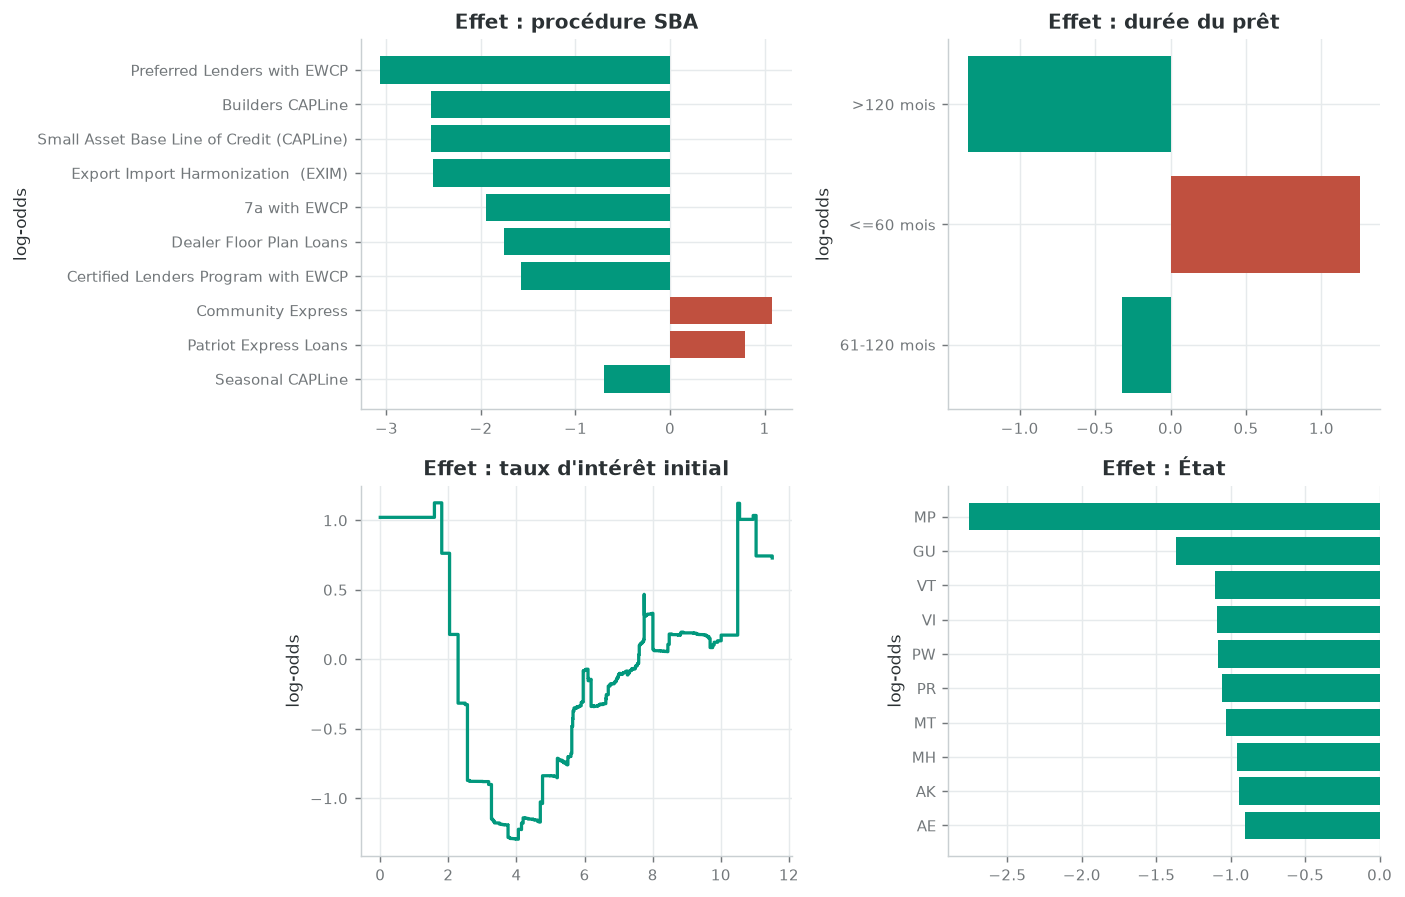
\includegraphics[width=\textwidth]{ebm_effets.png}
  \caption{Effet des quatre variables principales de l'EBM, en log-cote (rouge : augmente le risque ; vert : le
  réduit).}
  \label{fig:effets}
\end{figure}

\paragraph{Analyse des erreurs.} Au seuil qui maximise le F1, le modèle manque une majorité des défauts : le taux de
faux négatifs va de 57\,\% à 100\,\% selon l'État, et dépend fortement de la procédure (tableau~\ref{tab:erreurs}).
Pour les prêts des prêteurs certifiés, dont le taux de défaut est faible, presque aucun défaut n'est détecté. Le modèle
est donc un outil pour \emph{estimer et ordonner} un risque, pas pour détecter chaque défaut : c'est l'usage que nous en
faisons, puisque le MCDA utilise la probabilité et non une prédiction binaire.

\begin{table}[htbp]
\centering
\footnotesize\setlength{\tabcolsep}{4pt}
\caption{Analyse des erreurs de l'EBM par procédure (validation, seuil F1)}\label{tab:erreurs}
\begin{tabular}{lcccc}
\toprule
Procédure SBA & Prêts & Taux réel & PD moyenne & Faux négatifs \\
\midrule
SBA Express Program & 41\,517 & 4,0\,\% & 4,4\,\% & 61\,\% \\
Preferred Lenders Program & 20\,337 & 2,1\,\% & 2,0\,\% & 100\,\% \\
Small Loan Advantage Initiative & 9\,844 & 5,2\,\% & 3,6\,\% & 92\,\% \\
7a General & 5\,680 & 2,4\,\% & 2,5\,\% & 99\,\% \\
Patriot Express Loans & 1\,218 & 7,4\,\% & 6,7\,\% & 77\,\% \\
Working Capital CAPLine & 884 & 1,9\,\% & 2,0\,\% & 100\,\% \\
\bottomrule
\end{tabular}
\end{table}


% ---------------------------------------------------------------------------------------------
\section{Décision multicritère}

\subsection{Poids et filtre}

Les poids issus de l'AHP sont très proches des poids cibles (figure~\ref{fig:poids}), avec un ratio de cohérence de
0,009, bien inférieur au seuil de 0,10 ($\lambda_{\max} = 8{,}091$). Le filtre éliminatoire écarte 11 projets sur 40 :
8 pour un DSCR inférieur à 1 et 3 pour une probabilité de défaut supérieure à 7,1\,\%.

\begin{figure}[htbp]
  \centering
  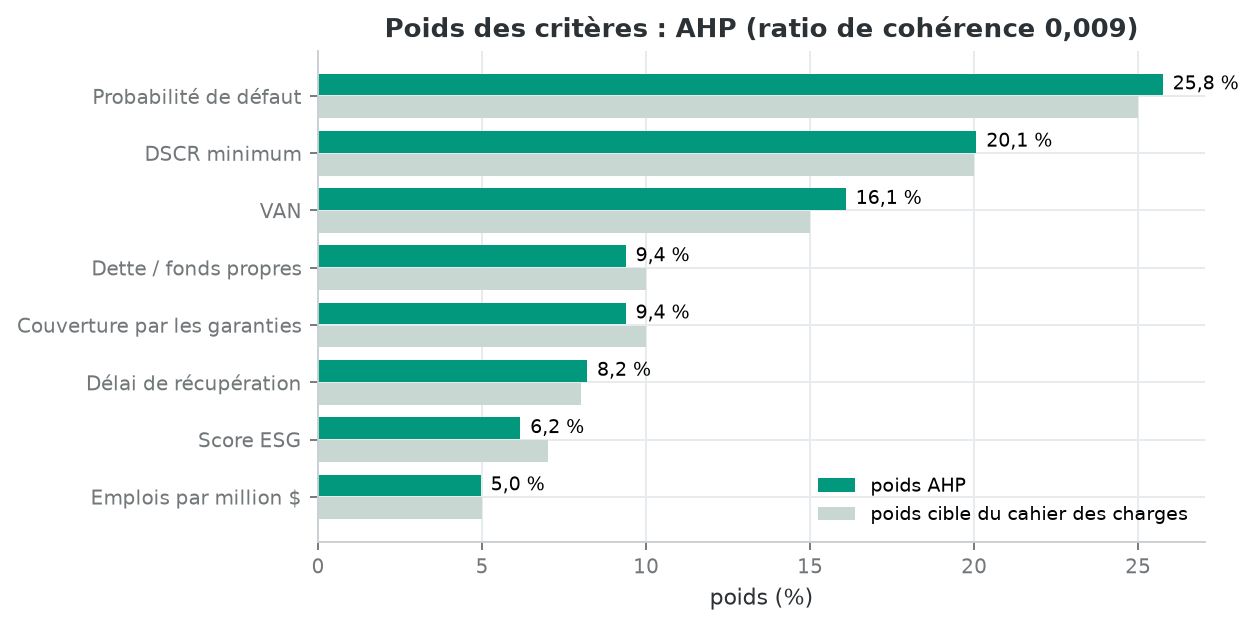
\includegraphics[width=0.8\textwidth]{mcda_poids.png}
  \caption{Poids des critères obtenus par AHP, comparés aux poids cibles.}
  \label{fig:poids}
\end{figure}

\subsection{Catégories et classement}

ELECTRE TRI (règle pessimiste, $\lambda = 0{,}6$) affecte \textbf{9 projets à \og Financer \fg{}, 19 à \og Financer
sous conditions \fg{} et 12 à \og Refuser \fg{}} (dont les 11 écartés par le filtre). La figure~\ref{fig:carte} situe
les 40 projets selon leur risque et leur DSCR : les projets à financer se concentrent dans la zone de faible risque et
de DSCR confortable, mais la catégorie dépend aussi des six autres critères, ce qui explique que des projets voisins
sur ce graphique soient classés différemment. Le classement ELECTRE III place en tête le Studio de développement
logiciel Murphy, l'Atelier d'insertion professionnelle Foster, le Bureau d'ingénierie Dubois, l'Entreprise de travaux
spécialisés Brooks et la Brasserie artisanale Garcia. La liste complète figure en annexe (tableau~\ref{tab:projets}).

\begin{figure}[htbp]
  \centering
  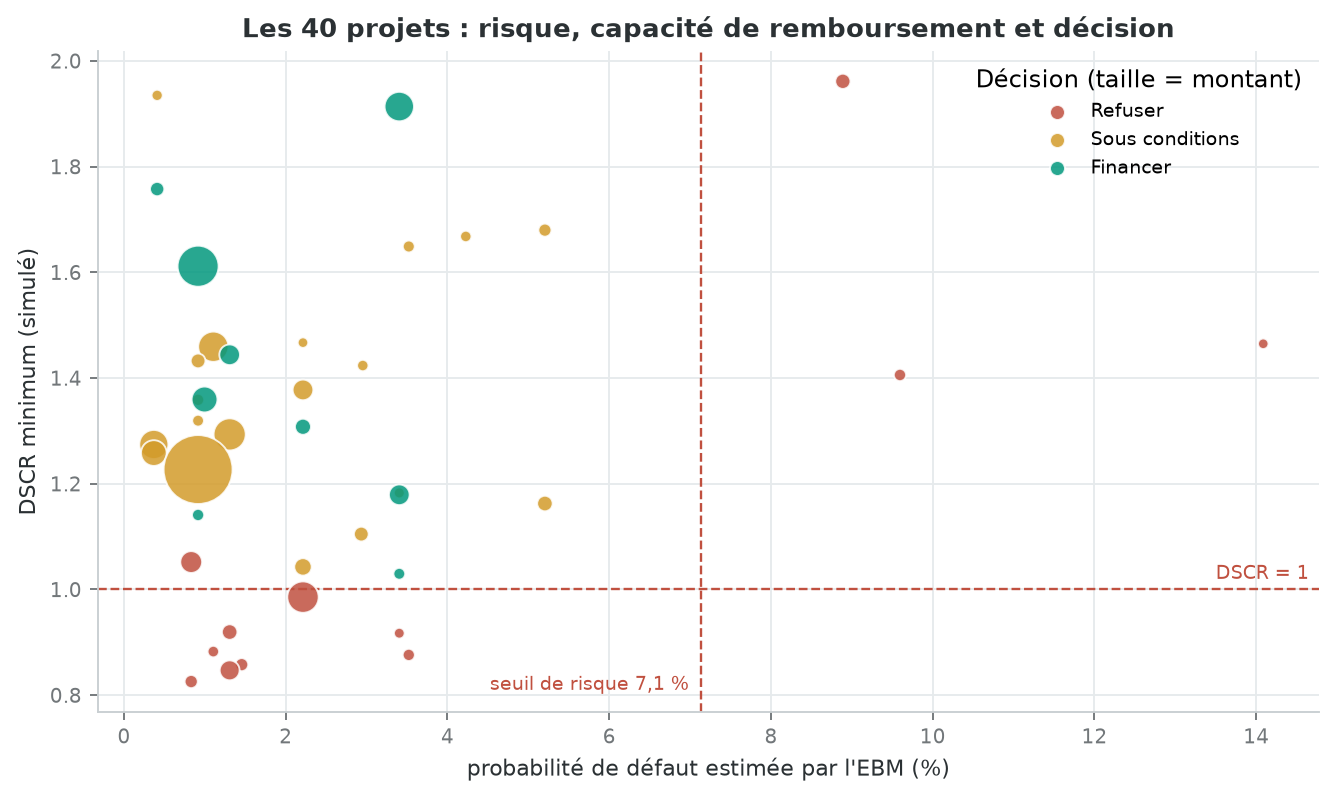
\includegraphics[width=0.9\textwidth]{mcda_carte.png}
  \caption{Les 40 projets selon leur probabilité de défaut et leur DSCR minimum ; couleur : décision ELECTRE TRI ;
  taille : montant demandé ; pointillés : seuils du filtre.}
  \label{fig:carte}
\end{figure}

Deux observations illustrent l'intérêt des méthodes de surclassement. Le Cabinet dentaire Baker a un risque très faible
(0,4\,\%) et un excellent score ESG, mais une VAN négative et un délai de récupération de 12,7 ans : il n'est que
\og sous conditions \fg{}, ses points forts ne compensant pas ses faiblesses. Par ailleurs, 7 projets ont une
\og position ambiguë \fg{} : les distillations descendante et ascendante les placent très différemment, ce qui signale
qu'ils sont incomparables à une partie des autres. Enfin, les règles pessimiste et optimiste d'ELECTRE TRI diffèrent
pour 15 projets : la règle pessimiste, retenue, est la plus prudente.

\subsection{Accord entre ELECTRE III et PROMETHEE II}

Les deux méthodes donnent des classements très proches pour les 29 projets non écartés (figure~\ref{fig:e3p2}) :
coefficient de Spearman de 0,891 et $\tau$ de Kendall de 0,724. Le classement ne dépend donc pas de façon critique de
la méthode choisie ; les écarts concernent surtout le milieu du classement, où les projets sont proches.

\begin{figure}[htbp]
  \centering
  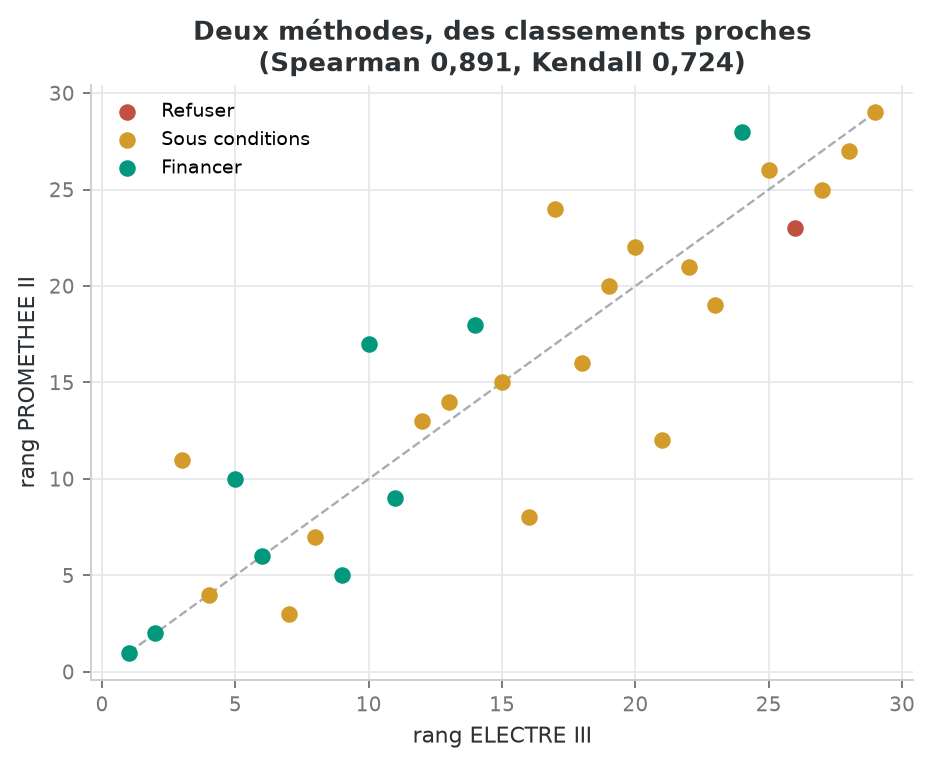
\includegraphics[width=0.55\textwidth]{mcda_e3_p2.png}
  \caption{Rangs ELECTRE III et PROMETHEE II des 29 projets non écartés.}
  \label{fig:e3p2}
\end{figure}

\subsection{Robustesse}

\paragraph{Un paramètre à la fois.} Le classement ELECTRE III bouge peu quand on modifie les seuils (Spearman de 0,937 à
0,976). Les catégories, elles, dépendent surtout de la coupure $\lambda$ (tableau~\ref{tab:sensibilite},
figure~\ref{fig:lambda}) : entre 0,5 et 0,8, 0 à 3 projets changent de catégorie, mais 10 changent à $\lambda = 0{,}9$
et 26 à $\lambda = 1$, valeur qui exige l'unanimité des critères. Un veto large ($v = 80\,\%$) modifie aussi 16
catégories.

\begin{table}[htbp]
\centering
\footnotesize\setlength{\tabcolsep}{4pt}
\caption{Sensibilité « un paramètre à la fois » (référence : q/p/v = 5/20/50\,\%, $\lambda$ = 0,6)}\label{tab:sensibilite}
\begin{tabular}{llccc}
\toprule
Paramètre & Valeur & Spearman & Kendall & Changements de catégorie \\
\midrule
Seuils q/p/v & 3\%/15\%/40\% & 0,937 & 0,793 & 4 \\
Seuils q/p/v & 5\%/20\%/50\% & 1,000 & 1,000 & 0 \\
Seuils q/p/v & 10\%/30\%/60\% & 0,976 & 0,882 & 8 \\
Seuils q/p/v & 5\%/20\%/80\% & 0,966 & 0,862 & 16 \\
Coupure $\lambda$ & 0,5 & 1,000 & 1,000 & 1 \\
Coupure $\lambda$ & 0,6 & 1,000 & 1,000 & 0 \\
Coupure $\lambda$ & 0,7 & 1,000 & 1,000 & 0 \\
Coupure $\lambda$ & 0,8 & 1,000 & 1,000 & 3 \\
Coupure $\lambda$ & 0,9 & 1,000 & 1,000 & 10 \\
Coupure $\lambda$ & 1 & 1,000 & 1,000 & 26 \\
\bottomrule
\end{tabular}
\end{table}


\begin{figure}[htbp]
  \centering
  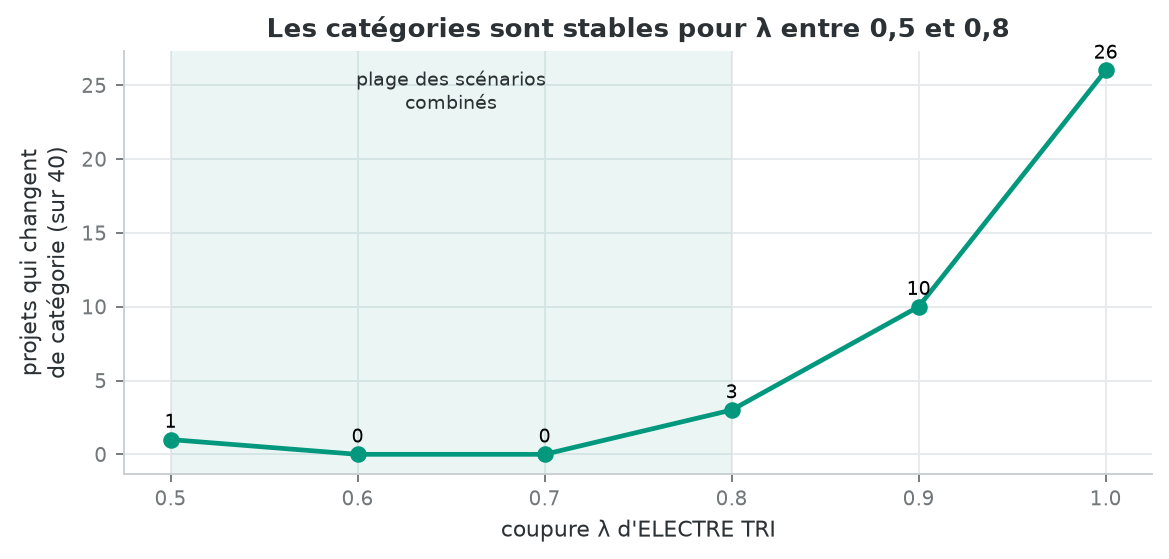
\includegraphics[width=0.75\textwidth]{mcda_lambda.png}
  \caption{Nombre de projets qui changent de catégorie selon la coupure $\lambda$.}
  \label{fig:lambda}
\end{figure}

\paragraph{Scénarios combinés et simulation.} Sur 200 scénarios faisant varier ensemble les poids, les seuils et
$\lambda$ (entre 0,5 et 0,8), 10 décisions sur 40 sont fragiles : 9 \og sous conditions \fg{} et 1 \og Refuser \fg{},
aucune parmi les \og Financer \fg{}. Les décisions de financement sont donc robustes aux paramètres de la méthode.
En revanche, avec les mêmes 40 prêts et 20 autres tirages des indicateurs simulés, un projet ne garde sa catégorie que
dans 48\,\% des cas en moyenne (figure~\ref{fig:stabilite}) : les catégories dépendent autant de la simulation que des
projets. C'est la principale limite de la démonstration, et la raison d'être de l'outil réutilisable, qui permet
d'appliquer la même méthode à des indicateurs réels.

\begin{figure}[htbp]
  \centering
  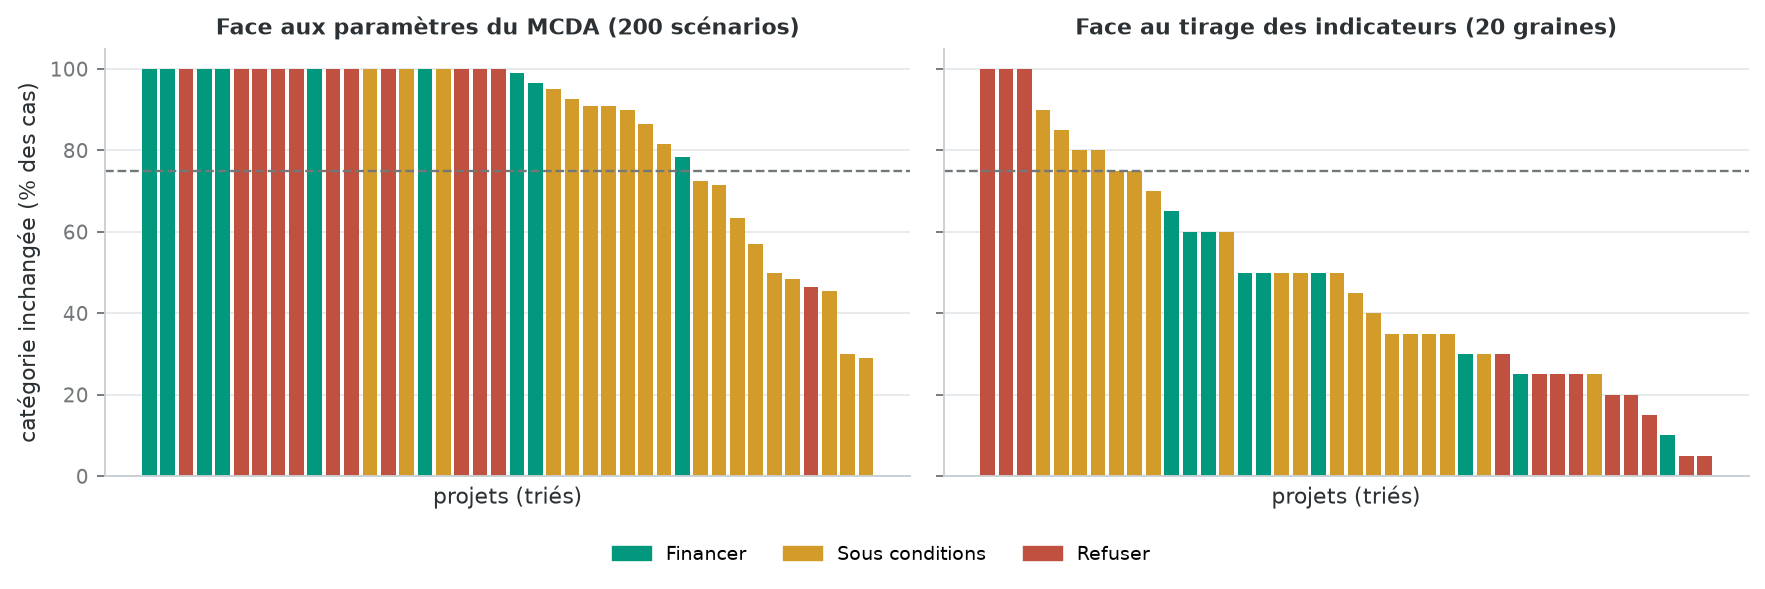
\includegraphics[width=\textwidth]{mcda_stabilite.png}
  \caption{Part des cas où la catégorie de chaque projet est inchangée : face aux paramètres du MCDA (gauche) et face
  au tirage des indicateurs simulés (droite).}
  \label{fig:stabilite}
\end{figure}

% ---------------------------------------------------------------------------------------------
\section{Arbitrage sous budget}

Avec un budget de 5\,M\$, la règle \og suivre le classement \fg{} retient \textbf{11 projets} (8 \og Financer \fg{} et
3 \og sous conditions \fg{}) pour 4,98\,M\$ engagés, soit 99,6\,\% du budget, répartis sur 7 secteurs
(figure~\ref{fig:arbitrage}). Un seul projet \og Financer \fg{} n'est pas retenu, les Pompes funèbres Price, parce que
son secteur atteint déjà le plafond de 35\,\% avec le Studio Murphy. Trois projets sont hors des bornes de montant,
dont le Garde-meubles Grant (5\,M\$, soit la totalité du budget).

\begin{figure}[htbp]
  \centering
  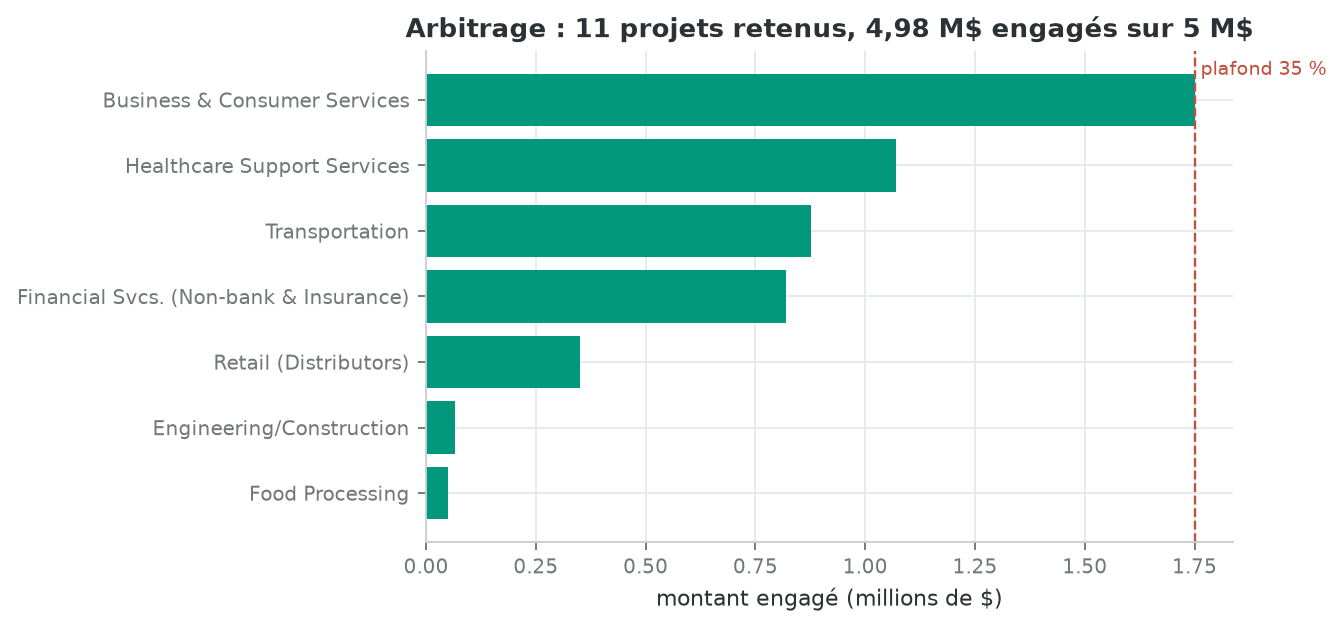
\includegraphics[width=0.85\textwidth]{arbitrage_secteurs.png}
  \caption{Montant engagé par secteur (règle \og suivre le classement \fg{}) ; pointillés : plafond sectoriel.}
  \label{fig:arbitrage}
\end{figure}

Le tableau~\ref{tab:arbitrage-regles} compare les deux règles. Maximiser le nombre de projets en finance 21 dans 11
secteurs, mais écarte le projet classé premier, le Studio Murphy (1,7\,M\$), au profit de plusieurs petits projets.
Ce résultat montre que l'objectif de l'optimisation n'est pas un détail technique : il traduit une politique. Nous
retenons par défaut la règle qui respecte le classement du comité, et proposons l'autre comme éclairage.

\begin{table}[htbp]
\centering
\small\setlength{\tabcolsep}{4pt}
\caption{Comparaison des deux règles de sélection (budget 5\,M\$, 20\,000 à 2\,M\$ par projet, 35\,\% au plus par secteur)}\label{tab:arbitrage-regles}
\begin{tabular}{lccccccc}
\toprule
Règle & Retenus & Financer & Sous cond. & Engagé & Utilisation & Secteurs & N\textsuperscript{o}\,1 financé \\
\midrule
Suivre le classement & 11 & 8 & 3 & 4,98\,M\$ & 99,6\,\% & 7 & oui \\
Maximiser le nombre & 21 & 8 & 13 & 4,89\,M\$ & 97,8\,\% & 11 & \textbf{non} \\
\bottomrule
\end{tabular}
\end{table}


% ---------------------------------------------------------------------------------------------
\section{Contrôle a posteriori}

Parmi les 40 prêts de démonstration, 3 ont réellement fait défaut dans les 60 mois. Les trois sont classés
\og Refuser \fg{} ; aucun des 9 projets \og Financer \fg{} ni des 19 \og sous conditions \fg{} n'a fait défaut.
La vraie issue n'est lue qu'après les décisions et n'entre dans aucun calcul. Avec trois cas, ce résultat est une
illustration encourageante, pas une preuve.
